% ==========================================================================
% = HES-SO Master thesis title page (modeled after Word template, 2016-2017)
% ==========================================================================

\begin{titlepage}
\newgeometry{margin=2cm}
{\fontfamily{phv}\fontseries{mc}\selectfont
    \begin{center}
	    
\includegraphics[width=0.95\textwidth]{img/heiafr_logo}
		~\\[1.5cm]
		% Title
		{
			\Huge
			PS5 - \ThesisTitle\\Rapport de projet \\[0.5cm]
			\large Informatique et Système de Communication (ISC), 2022-2023\\[2cm]
		}
		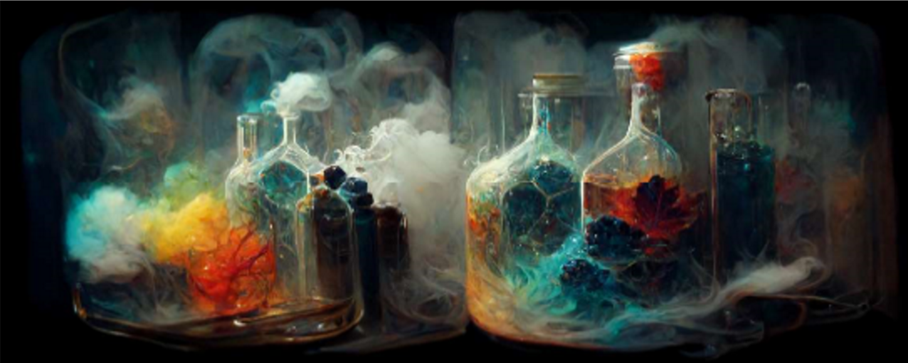
\includegraphics[width=0.8\textwidth]{img/logo.png}
		~\\[2cm]
		% Info
		{
			\begin{center}
			\begin{tabularx}{\textwidth} { %tableau pour créer 2 colonnes 
				>{\raggedright\arraybackslash}X 
				>{\raggedright\arraybackslash}X  }
					 \textbf{Etudiant} & \Author\\
					 & \\
					 \textbf{Enseignants responsables} & \Advisor \space - \AdvisorSchool \\ & \AdvisorTwo \space - \AdvisorTwoSchool \\
					 & \\
					 \textbf{Mendant} & \MendantInstitut \\ & \MendantOne \space - \MendantOneSchool \\ & \MendantTwo \space - \MendantTwoSchool\\
			\end{tabularx}
			\end{center}
			~\\[1.5cm]
		}
%		{
%			\large
%			External expert: \\
%			\Expert
%		}

        % {
        % Le code de ce projet est disponible en open source avec l'accord de tous ses
        % participants.
        % }
		\vfill
		
		 
		
		% Bottom of the page
	    {\projectVersion}\\
		{\large \Place, HEIA-FR, \Date}
		
	\end{center}
}
\restoregeometry
\end{titlepage}




